\documentclass[paper=a4, fontsize=11pt]{scrartcl} % A4 paper and 11pt font size

\usepackage[T1]{fontenc} % Use 8-bit encoding that has 256 glyphs
\usepackage{fourier} % Use the Adobe Utopia font for the document - comment this line to return to the LaTeX default
\usepackage[english]{babel} % English language/hyphenation
\usepackage{amsmath,amsfonts,amsthm,amssymb} % Math packages

\usepackage{algorithm, algorithmic}
\renewcommand{\algorithmicrequire}{\textbf{Input:}} %Use Input in the format of Algorithm  
\renewcommand{\algorithmicensure}{\textbf{Output:}} %UseOutput in the format of Algorithm  

\usepackage{graphicx}

\usepackage{listings}
\lstset{language=Matlab}

\usepackage{lipsum} % Used for inserting dummy 'Lorem ipsum' text into the template

\usepackage{sectsty} % Allows customizing section commands
\allsectionsfont{\centering \normalfont\scshape} % Make all sections centered, the default font and small caps

\usepackage{fancyhdr} % Custom headers and footers
\pagestyle{fancyplain} % Makes all pages in the document conform to the custom headers and footers
\fancyhead{} % No page header - if you want one, create it in the same way as the footers below
\fancyfoot[L]{} % Empty left footer
\fancyfoot[C]{} % Empty center footer
\fancyfoot[R]{\thepage} % Page numbering for right footer
\renewcommand{\headrulewidth}{0pt} % Remove header underlines
\renewcommand{\footrulewidth}{0pt} % Remove footer underlines
\setlength{\headheight}{13.6pt} % Customize the height of the header

\numberwithin{equation}{section} % Number equations within sections (i.e. 1.1, 1.2, 2.1, 2.2 instead of 1, 2, 3, 4)
\numberwithin{figure}{section} % Number figures within sections (i.e. 1.1, 1.2, 2.1, 2.2 instead of 1, 2, 3, 4)
\numberwithin{table}{section} % Number tables within sections (i.e. 1.1, 1.2, 2.1, 2.2 instead of 1, 2, 3, 4)

\setlength\parindent{0pt} % Removes all indentation from paragraphs - comment this line for an assignment with lots of text

%----------------------------------------------------------------------------------------
%	TITLE SECTION
%----------------------------------------------------------------------------------------

\newcommand{\horrule}[1]{\rule{\linewidth}{#1}} % Create horizontal rule command with 1 argument of height

\title{	
\normalfont \normalsize 
\textsc{Shanghai Jiao Tong University, UM-SJTU JOINT INSTITUTE} \\ [25pt] % Your university, school and/or department name(s)
\horrule{0.5pt} \\[0.4cm] % Thin top horizontal rule
\huge Methods of Applied Mathematics I\\ HW3 \\ % The assignment title
\horrule{2pt} \\[0.5cm] % Thick bottom horizontal rule
}

\author{Yu Cang \\ 018370210001} % Your name

\date{\normalsize \today} % Today's date or a custom date

\begin{document}

\maketitle % Print the title

\section{Exercise3.1}
	\begin{proof}
		Let $\phi(x) = (x^2 - 1)^n$, then
		\begin{equation}
			\phi(\pm 1) = \phi^{(1)}(\pm 1) = \cdots = \phi^{(n-1)}(\pm 1) = 0
		\end{equation}
		The $L^2$ norm of $P_n(x)$ is
		\begin{equation}
			\begin{aligned}
				||P_n||_2  & = \sqrt{\int_{-1}^{1} P_n^2(x) dx}\\
						   & = \sqrt{(\frac{1}{2^n n!})^2 \int_{-1}^{1} [\phi^{(n)}(x)]^2 dx}\\
						   & = \sqrt{(\frac{1}{2^n n!})^2 (-1)^n \int_{-1}^{1} \phi^{(2n)}(x) \phi(x) dx} \quad \text{(Integrate by parts)}\\
						   & = \sqrt{(\frac{1}{2^n n!})^2 (-1)^n (2n)! \int_{-1}^{1} (x^2 - 1)^n dx}\\
						   & = \sqrt{(\frac{1}{2^n n!})^2 (-1)^n (2n)! \cdot 2 \int_{0}^{\frac{\pi}{2}} (sin^2(x) - 1)^n cos(x) dx}\\
						   & = \sqrt{(\frac{1}{2^n n!})^2 (2n)! \cdot 2 \int_{0}^{\frac{\pi}{2}} cos^{2n+1}(x) dx}\\
			\end{aligned}
		\end{equation}
		Since
		\begin{equation}
			\int_{0}^{\frac{\pi}{2}} cos^{2n+1}(x) dx = \frac{2 \times 4 \times \cdots \times (2n)}{1\times3\times \cdots \times (2n+1)} 
		\end{equation}
		substitute it into the norm equation of $P_n$ yields
		\begin{equation}
			||P_n||_2 = \sqrt{(\frac{1}{2^n n!})^2 (2n)! \cdot 2 \cdot \frac{2 \times 4 \times \cdots \times (2n)}{1\times3\times \cdots \times(2n+1)}} = \sqrt{\frac{2}{2n+1}}
		\end{equation}
	\end{proof}

\section{Exercise3.2}
	\begin{enumerate}
		\item 
			Consider the projection of $f(x)$ onto $P_0(x)$, $P_1(x)$ and $P_2(x)$ correspondingly
			\begin{equation}
				(f, P_0) = \int_{-1}^{1} e^x dx = e - \frac{1}{e}
			\end{equation} 
			
			\begin{equation}
				(f, P_1) = \int_{-1}^{1} x e^x dx = \frac{2}{e}
			\end{equation}
			
			\begin{equation}
				(f, P_2) = \int_{-1}^{1} \frac{3x^2 -1}{2} e^x dx = e - \frac{7}{e}
			\end{equation}
			As $(P_i, P_j)=0$ when $i \neq j$, $p(x)$ can be written as linear combination of $P_i$
			\begin{equation}
				p(x) = a_0 P_0(x) + a_1 P_1(x) + a_2 P_2(x)
			\end{equation}
			with coefficient $a_i$ given as
			\begin{equation}
				a_i = \frac{(f, P_i)}{(P_i, P_i)} = \frac{2i+1}{2} (f, P_i)
			\end{equation}
			Finally
			\begin{equation}
				p(x) = 1.1752 P_0(x) + 1.1036 P_1(x) + 0.3578 P_2(x)
			\end{equation}
			
		\item 
		The plot(Fig \ref{fig:comp}) is provided for comparsion.
	
		\begin{figure}[!htbp]
			\centering
			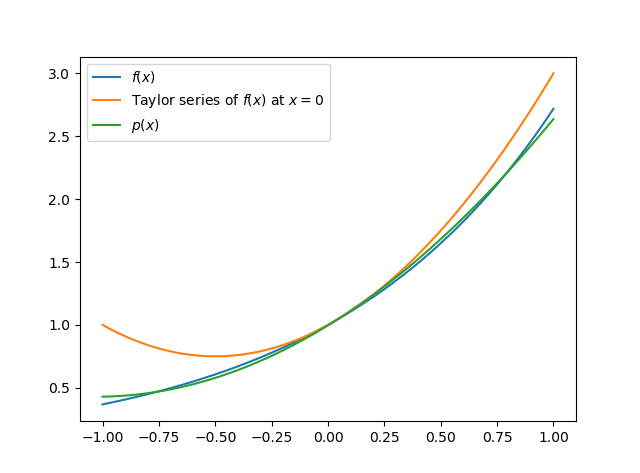
\includegraphics[]{ApproximationCompare.png}
			\caption{Comparsion of different approximation for $e^x$}
			\label{fig:comp}
		\end{figure}
	
		The distinction is quite obvious and Legendre polynomials does better than taylor series expansion at zero point.
	
	\end{enumerate}

\section{Exercise3.3}
	\begin{enumerate}
		\item 
		
		\item 
		
	\end{enumerate}

\end{document}